%- 
{% ------ COMPOSITE GRID ------
\def\rad{.5}% .8 
\newcommand{\plotDisk}{
% Plot the rigid body
\fill[fill=red!20,draw=red,line width=2pt] 
      plot[samples=100, domain=0.:360] ( {\rad*cos(\x)} , {\rad*sin(\x)} ) -- cycle ;
}
\newcommand{\figWidth}{8cm}
\newcommand{\figWidthz}{7cm}
\newcommand{\trimfig}[2]{\trimh{#1}{#2}{.4}{.4}{.02}{.02}}
\newcommand{\trimfiga}[2]{\trimh{#1}{#2}{.4}{.4}{.35}{.25}}
\newcommand{\trimfigz}[2]{\trimh{#1}{#2}{.0}{.075}{.0}{.0}}
% \newcommand{\labelsize}{\footnotesize}
\newcommand{\labelsize}{\small}
\begin{figure}[htb]
\begin{center}
\resizebox{12cm}{!}{% START resize box
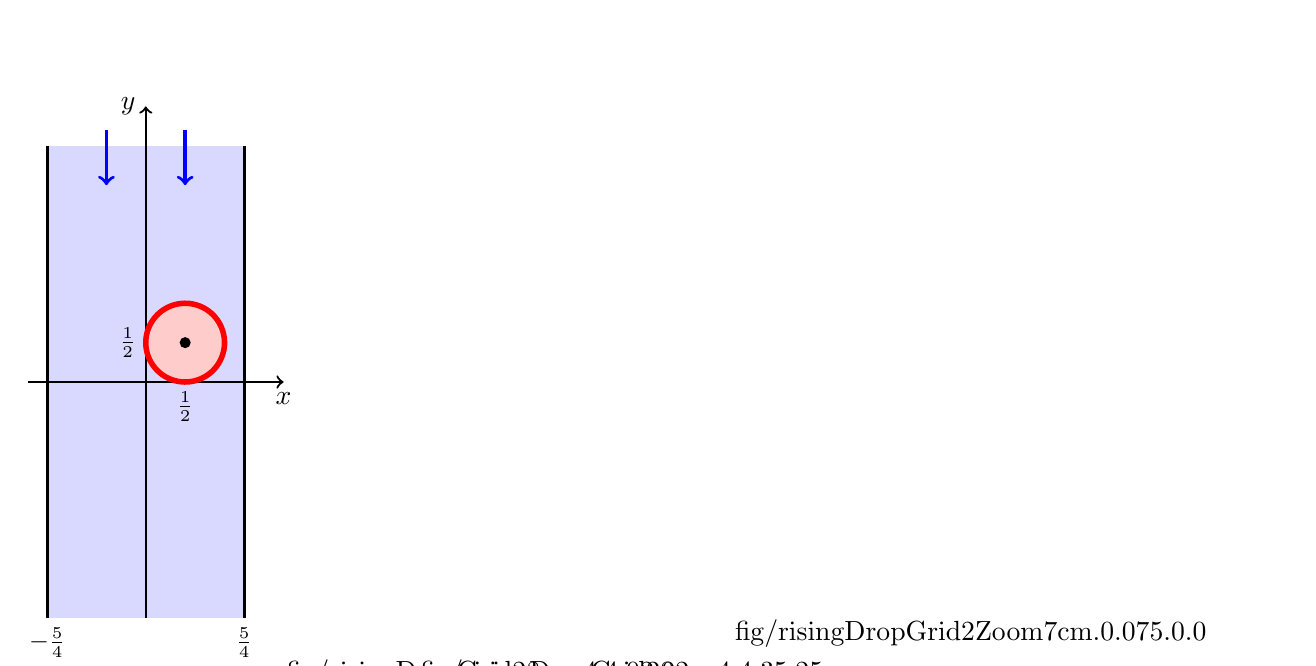
\begin{tikzpicture}[scale=1]
  \useasboundingbox (0.0,.75) rectangle (16.,8.5);  % set the bounding box (so we have less surrounding white space)
  % 
  \begin{scope}[xshift=1.5cm,yshift=4cm]
      \fill[fill=blue!15] (-1.25,-3) -- (1.25,-3) -- (1.25,3) -- (-1.25,3) -- cycle; 
      \draw[->,very thick,blue] (-.5,3.2) -- (-.5,2.5); 
      \draw[->,very thick,blue] (.5,3.2) -- (.5,2.5); 
      \draw[->,thick] (-1.5,0) -- (1.75,0) node [anchor=north] {$x$}; % x-axis
      \draw[->,thick] (0,-3) -- (0,3.5) node [anchor=east] {$y$}; % y-axis
      %
      \draw[-,very thick] (-1.25,-3) -- (-1.25,3);
      \draw[-,very thick] (1.25,-3) -- (1.25,3);
    % plot the disk
    \begin{scope}[xshift=.5cm,yshift=.5cm]  
      \plotDisk
    \end{scope}
    % \draw(0,0) node[anchor=north west] {\labelsize$\mathbf{0}$}; 
    \fill[black] (.5,.5) circle (2 pt); % center of disk
    \draw(.5,0) node[anchor=north] {\labelsize$\frac{1}{2}$}; 
    \draw(0,.5) node[anchor=east] {\labelsize$\frac{1}{2}$}; 
    \draw(-1.25,-3) node[anchor=north] {\labelsize$-\frac{5}{4}$};
    \draw( 1.25,-3) node[anchor=north] {\labelsize$\frac{5}{4}$};
    % \draw(-1.25,0) node[anchor=north west] {\labelsize$(-\frac{5}{4},0)$}; 
    % \draw( 1.25,0) node[anchor=south east] {\labelsize$(\frac{5}{4},0)$}; 
  \end{scope}
  % grids ---
  \draw(3.3,0) node[anchor=south west,xshift=-4pt,yshift=+0pt] {\trimfig{fig/risingDropGrid2}{\figWidth}};
  \draw(5.0,0) node[anchor=south west,xshift=-4pt,yshift=+0pt] {\trimfiga{fig/risingDropGrid2}{\figWidth}};
  \draw(9.0,.5) node[anchor=south west,xshift=-4pt,yshift=+0pt] {\trimfigz{fig/risingDropGrid2Zoom}{\figWidthz}};
%% \draw(8.0,0) node[anchor=south west,xshift=-4pt,yshift=+0pt] {\trimfig{fig/bic4Gridt1p0}{\figWidth}};
% grid:
% \draw[step=1cm,gray] (0,0) grid (16,8.);
\end{tikzpicture}
}% end resize box
\end{center}
  \caption{Rising disk in a counter-flow. Left: geometrical configuration at $t=0$.
  The other figures show the composite grid $\Gcrd^{(2)}$ (coarse grid), plus zooms.
%   Left: entire grid showing coarser inlet and outlet grids. Middle: partial zoom showing the grids
%  in the central portion of the computational domain. Right: zoom near the disk. 
%   The red fluid grid adjacent to the
%    rigid disk (solid red) moves in time. The blue and green fluid grids do not move.
}
  \label{fig:risingDiskGrid}
\end{figure}
}
